% Document template based on LNCS, adapted by Matt Welsh <mdw@cs.berkeley.edu>

% This version is adapted to use PDFTEX to render to PDF directly. 
% If you want to use dvi, you need to change any figures to use '.eps'
% rather than '.pdf', and probably get rid of the hyperref package.

\documentclass{article}
\usepackage{program}
\usepackage{acm-style10} % ACM proceedings formatting
\usepackage{times}       % Use Adobe Times font set
\usepackage{epsfig,twocolumn}
\usepackage{url}
\usepackage[english]{babel} % mdw: Required to get good hyphenation on RH6.0
                            % (fixed in RH6.1)
\usepackage{graphicx} 
\usepackage{color}

% DO NOT EDIT THE BELOW BLOCK OF CODE
\def\dsp{\def\baselinestretch{1.10}}
\dsp
\newcommand{\XXXnote}[1]{{\bf\color{red} XXX: #1}}
\setlength{\textheight}{9.25in}
\setlength{\columnsep}{0.33in}
\setlength{\textwidth}{7.4in}
\setlength{\footskip}{0.0in}
\setlength{\topmargin}{-0.25in}
\setlength{\headheight}{0.0in}
\setlength{\headsep}{0.0in}
\setlength{\oddsidemargin}{-.45in}
\setlength{\parindent}{1pc}
\pagestyle{empty}
\begin{document}
\date{}

%%%%%%%%%%%% THIS IS WHERE WE PUT IN THE TITLE AND AUTHORS %%%%%%%%%%%%

% Title here
\title{\ttlfnt Achieving Synchronicity in Wireless Sensor Networks}

% Author names, affiliations, and e-mail below
\author{{\aufnt  Uri Braun, Geetika Tewari, Geoffrey Werner-Allen} \\ 
{\affaddr Harvard University} \\ 
{\affaddr { \{uribraun, gtewari, werner\}}@eecs.harvard.edu}}

\maketitle
%\copyrightspace
\thispagestyle{empty}

%%%%%%%%%%%%%  ABSTRACT GOES HERE %%%%%%%%%%%%%%

\subsection*{Abstract}
\begin{small}
Synchronicity can play an important role in facilitating tasks such as 
power minimization, data logging, time synchronization, and event detection 
in wireless sensor networks.
Achieving synchronicity in sensor networks is challenging due to their
characteristic limited node resources and communication bandwidth, node crystal frequency variations, 
and lossy communication links across multi-hop networks.

We investigate the accuracy and quality of synchronicity achieved in 
a network of wireless sensors that is inspired from synchrony observed in swarms
of biological systems such as that of synchronous fireflies or spiking of neurons.
We emulate the pulse coupled integrate and fire model embedded
in such biological swarms that is guaranteed to converge by the theory proposed
by Mirollo and Strogatz~\cite{ms90}.
Our work is motivated by a variety of recent work that demonstrates the effectiveness
of this model in wireless sensor networks. 
Hong, Cheow and Scaglione use this model to propose schemes for distributed time synchronization 
and change detection in wireless sensors networks~\cite{hcs04,tsrbc03,ssp03}.
More compelling is recent work by Lucarelli and Wang~\cite{lw04} that builds upon this, and defines 
a class of models that can converge to a synchronized state based on purely local
interactions amongst nodes in sensor networks, and thus lifts the all-to-all 
communication requirement assumed in Mirollo and Strogatz's model and 
implicit in~\cite{hcs04,tsrbc03,ssp03}

In this paper, we design a variant of Mirollo and Strogatz's 
model of synchronicity for wireless sensor networks that does not assume 
all-to-all communication.
We implement and evaluate our synchronicity algorithm on Motelab, a 38 node
cluster of MicaZ sensors deployed in the Harvard Computer Science building,
as well as on TOSSIM, a TinyOS mote simulator~\cite{hill00}.
\end{small}

%%%%%%%%%%%%%  BODY OF PAPER %%%%%%%%%%%%%%

\section{Introduction}

Computer scientists have often looked to nature for inspiration.
Researchers studying distributed systems have long envied, and
attempted to duplicate, the fault-tolerance and decentralized control
achieved in natural systems.  Those of us studying sensor networks
also have every reason to be envious.  Designing software coordinating
the output of a collection of limited devices frequently feels as
frustrating as orchestrating the activity of a colony of stubborn
ants, or guiding a school of uncooperative fish.  And yet ant colonies
complete difficult tasks, schools of fish navigate the sea, and swarms
of fireflies stretching for miles can pulse in perfect unison, all
without centralized control or perfect individuals. The spontaneous
emergence of synchronicity --- for example, fireflies flashing in
unison or cardiac cells firing in synchrony --- has long attracted the
attention of biologists, mathematicians and computer scientists.

%% SIMULTANEOUS COLLECTIVE ACTION

Synchronicity is a powerful primitive for sensor networks. We define
synchronicity as the ability to organize {\em simultaneous collective
action} across a sensor network. Synchronicity is not the same as time
synchronization: the latter implies that nodes share a common notion
of time that can be mapped back onto a real-world clock, while the
former only requires that nodes agree on a firing period and phase.
The two primitives are complementary: nodes with access to a common
time base can schedule collective action in the future, and
conversely, nodes that can arrange collective action can establish a
meaningful network-wide time base. However, the two primitives are also
independently useful. For example, nodes within a sensor network may
want to compare the times at which they detected some event. This task
requires a notion of global time, however it does not require
real-time coordination of actions. 

Similarly, synchronicity by itself can be extremely useful as a sensor
network coordination primitive. A commonly-used mechanism for limiting
energy use is to carefully schedule node duty cycles so that all nodes
in a network (or a portion of the network) will wake up at the same
time, sample their sensors, and relay data along a routing path to the
base station. Coordinated communication scheduling has been used both
at the MAC level~\cite{s-mac} and in multi-hop routing
protocols~\cite{stem} to save energy. Synchronicity can also be
used to coordinate sampling across multiple nodes in a network,
which is especially important in applications with high data
rates. Previous work on seismic analysis of
structures~\cite{glaser-smart-buildings}, shooter
localization~\cite{shooter-localization}, and volcanic
monitoring~\cite{volcano-ewsn05} could use such a primitive and avoid
the overhead of maintaining consensus on global time until
absolutely necessary.

In this paper, we present a biologically-inspired distributed
synchronicity algorithm implemented on TinyOS motes. This algorithm is
based on a mathematical model originally proposed by Mirollo and
Strogatz to explain how neurons and fireflies spontaneously
synchronize~\cite{strogatz}. This seminal work proved that a very
simple reactive node behavior would always converge to produce global
synchronicity, irrespective of the number of nodes and starting
times. Recently Lucarelli and Wang~\cite{lucarelli04} demonstrated
that this result also holds for multi-hop topologies, an important
contribution towards making the model feasible for sensor networks.

The firefly-inspired synchronization described by Mirollo and Strogatz
has several salient features that make it attractive for sensor
networks. Nodes execute very simple computations and interactions, and
maintain no internal state regarding neighbors or network topology. As
a result, the algorithm robustly adapts to changes such as the loss
and addition of nodes and links \cite{lucarelli04}. The synchronicity
provably emerges in a completely decentralized manner, without any
explicit leaders and irrespective of the starting state.

However, implementing this approach on wireless sensor networks still
presents significant obstacles. In particular, the previous
theoretical work assumes {\em instantaneous} communication between
nodes.  In real sensor networks, radio contention and processing
latency lead to significant and unpredictable communication
latencies. Earlier work also assumes non-lossy radio links, identical
oscillator frequencies, and arbitrary-precision floating-point
arithmetic which are unrealistic in current sensor networks.

We present the {\em reachback firefly algorithm} (RFA) that accounts for
communication latencies, by modifying the original firefly model to
allow nodes to use information from the past to adjust the future
firing phase. We evaluate our algorithm in three ways: theory,
simulation and implementation. We present theoretical results to prove
the convergence of our algorithm in simple cases and predict the
impact of parameter choice. Next we leverage TOSSIM, the TinyOS
simulator, to explore the behavior of the algorithm over a range of
parameter values, varying numbers of nodes, and different
communication topologies. These simulation results validate the
theoretical predictions. Finally, we present results from experiments
on a real sensor network testbed. These results demonstrate that our
algorithm is robust in the face of real radio effects and node
limitations.  Our results show that such a decentralized approach can
provide synchronicity to within 100~$\mu$sec on a complex multiple-hop
network with asymmetric and lossy links. To the best of our knowledge,
this work represents the first implementation of firefly-inspired
synchronicity on the MicaZ mote hardware, and demonstrates the ability
of the model to achieve synchronicity given real radio and hardware
limitations.

Our paper is organized as follows. Section \ref{sec-background}
presents related work. In Section \ref{sec-algorithm} we present RFA
in the context of the Mirollo and Strogatz model and describe current
hardware and radio limitations. Sections
\ref{sec-theory}-\ref{sec-motes} present our metrics and theoretical,
simulation and experimental results. We conclude with future work.



 
\section{Background and Motivation}
\label{sec-background}

Time synchronization has received a great deal of attention in the
sensor network community. The problem of establishing a consistent global
timebase across a large network, despite message loss and delays, node
failures, and local clock skew, has proven to be very difficult. As
described in the introduction, our goal is not time synchronization,
but rather {\em synchronicity:} the ability for all nodes in the
network to agree on a common period and phase for firing
pulses. Synchronicity can be used to implement time synchronization,
although this requires mapping the local firing cycle to a
global clock, which we leave for future work. 

%% not quite true
%% For example, the Flooding Time Synchronization Protocol (FTSP)~\cite{ftsp}
%% uses multiple rounds of message transmission on each synchronization
%% cycle to accurately estimate clock skew and message delays. In cases
%% where only synchronicity is required, this overhead may not be desirable.

%% mostly moved to introduction
%% Synchronicity without time synchronization is extremely useful as a 
%% sensor network coordination primitive. A commonly-used mechanism for
%% limiting energy use is to carefully schedule node duty cycles so that
%% all nodes in a network, or a portion of the network, will wake up at
%% the same time, sample their sensors, and relay data along a routing
%% path to the base station. Coordinated communication scheduling 
%% has been used both at the MAC level~\cite{t-mac,s-mac} and in 
%% multihop routing protocols~\cite{leach,stem} to save 
%% energy.

%% Synchronicity can also be used to correlate signals across multiple
%% nodes in a network, which is especially important in applications
%% with high data rates. Previous work on seismic analysis of
%% structures~\cite{glaser-smart-buildings,wisan}, shooter
%% localization~\cite{shooter-localization}, and volcanic 
%% monitoring~\cite{volcano-ewsn05} could use a synchronicity primitive, 
%% rather than time synchronization, to establish signal correlation
%% across sensor nodes.

\subsection{Time Synchronization}

%Time synchronization in sensor networks is a well-studied problem.

A number of protocols have been proposed that allow wireless sensor
nodes to agree on a common global timebase. Here we briefly describe
some of the protocols. In Receiver Based Synchronization
(RBS)~\cite{rbs} a reference node broadcasts a message and multiple
receivers within radio range can then agree on a common time base by
exchanging the local clock times at which they received the message.
This protocol avoids the uncertainty of transmission delays by using a
single radio message to simultaneously synchronize multiple receiver
nodes, however it does not apply in multi-hop networks. The
TPSN~\cite{tpsn} protocol works on multi-hop networks by constructing
a spanning tree and then using hop-by-hop synchronization along the
edges to synchronize all nodes to the root. They also introduce MAC
level timestamping to estimate transmission delay. The FTSP
protocol \cite{ftsp}, simplifies the process of multi-hop
synchronization by using periodic floods from an elected root, rather
than maintaining a spanning tree. In the case of root failure, the
system elects a new root node. FTSP also refines the timestamping
process to within microsecond accuracy and provides a method for
estimating clock drift which reduces the need to synchronize
frequently.

Direct comparison of these protocols in terms of synchronization error
is difficult, due to the differences in hardware and evaluation
methodology. FTSP reports a per-hop synchronization error of about
1~$\mu$sec, although the maximum pairwise error is over 65~$\mu$sec in
their testbed.  The mean single-hop synchronization error reported for
TPSN is 16.9~$\mu$sec, compared to 29.1~$\mu$sec for RBS~\cite{tpsn}.
The dynamics of these protocols in terms of robustness to topology
changes and node population have not been widely studied.

\subsection{Biologically-Inspired Synchronicity}

Synchronicity has been observed in large biological swarms where
individuals follow simple coordination strategies. The canonical
example is the synchrony of fireflies observed in certain parts of
southeast Asia~\cite{strogatz}.  The behavior of these systems can be
modeled as a network of {\em pulse-coupled oscillators} where each
node is an oscillator that periodically emits a self-generated pulse.
Upon observing other oscillators' pulses, a node adjusts the phase of
its own oscillator slightly. This simple feedback process results in
the nodes tightly aligning their phases and achieving synchronicity.

Peskin first introduced this model in the context of cardiac pacemaker
cells\cite{peskin75}. Mirollo and Strogatz~\cite{strogatz} provide one
of the earliest complete analytical studies of pulse-coupled
oscillator systems. They proved that a fully-connected (all-to-all)
network of $N$ identical pulse-coupled oscillators would synchronize,
for any $N$ and any initial starting times. Recent work by Lucarelli
and Wang~\cite{lucarelli04} relaxes the all-to-all communication
assumption. Drawing from recent results in multi-agent control, they
derive a stability result based on nearest neighbor coupling and show
convergence in simulation for static and time varying
topologies. Their work demonstrates that the same simple feedback
process works, even when nodes only observe nearest neighbors and
those neighbors may change over time.

Several groups have proposed using pulse-coupled synchronicity to
solve various network problems. Hong and
Scaglione~\cite{tsrbc03,hcs04} introduce an adaptive distributed time
synchronization method for fully-connected Ultra Wideband (UWB)
networks. They use this as a basis for change detection
consensus. Wakamiya and Murata~\cite{wm04} propose a scheme for data
fusion in sensor networks where information collected by sensors is
periodically propagated without any centralized control from the edge
of a sensor network to a base station, using pulse-coupled
synchronicity. Wokoma et al.~\cite{wl02} propose a weakly coupled
adaptive gossip protocol for active networks. Each
of these applications clearly demonstrates the utility of
synchronicity as a primitive. However much of the prior work is
evaluated only in simulation and does not consider real communication
delay or loss.

Wireless radios exhibit non-negligible and unpredictable delays due to
channel coding, bit serialization, and (most importantly) backoff at
the MAC layer \cite{tpsn,ftsp}. In traditional CSMA MAC schemes, a
transmitter will delay a random interval before initiating
transmission once the channel is clear. Additional random (typically
exponential) backoffs are incurred during channel contention.  On the
receiving end, jitter caused by interrupt overhead and packet
deserialization leads to additional unpredictable delays.  Radio
contention deeply impacts the firefly model.  Multiple nodes
attempting to fire simultaneously will be unable to do so by the very
nature of the CSMA algorithm. As nodes achieve tighter synchronicity,
contention will become increasingly worse as many nodes attempt to
transmit simultaneously. The goal of this paper is to address the
limitations of current communication assumptions and realize a real
implementation of firefly-inspired synchronicity in sensor networks.

%% The simplicity of the pulse-coupled oscillator model and the parallel
%% between the limited capabilities of fireflies and sensor nodes,
%% provides an excellent motivation for investigating it as a
%% synchronicity algorithm for wireless sensor nodes. 

%% While their theoretical and simulation results are promising, their
%% model inherently assumes that radio communication is instantaneous,
%% and that nodes can instantaneously observe and react to neighbors
%% firing. They also assume that an arbitrary number of nodes can
%% transmit messages simultaneously when they fire.

%% Our work represents the first
%% implementation of firefly-inspired synchronicity on the MicaZ mote
%% hardware, and demonstrates the ability of the model to achieve tight
%% synchronicity given real radio and hardware limitations. 


\section{Implementing FICA in Wireless Sensor Networks}
\label{sec:fits}

Significant changes were necessary to adapt the original Strogatz
coupled-oscillators model for use on wireless sensor nodes.  Because
Strogatz's model is well documented in the literature we offer only a brief
description here.  We then continue this section detailing the challenges
created by assumptions in the model untenable on real systems and describing
our solutions.

\begin{figure}[t]
\begin{center}
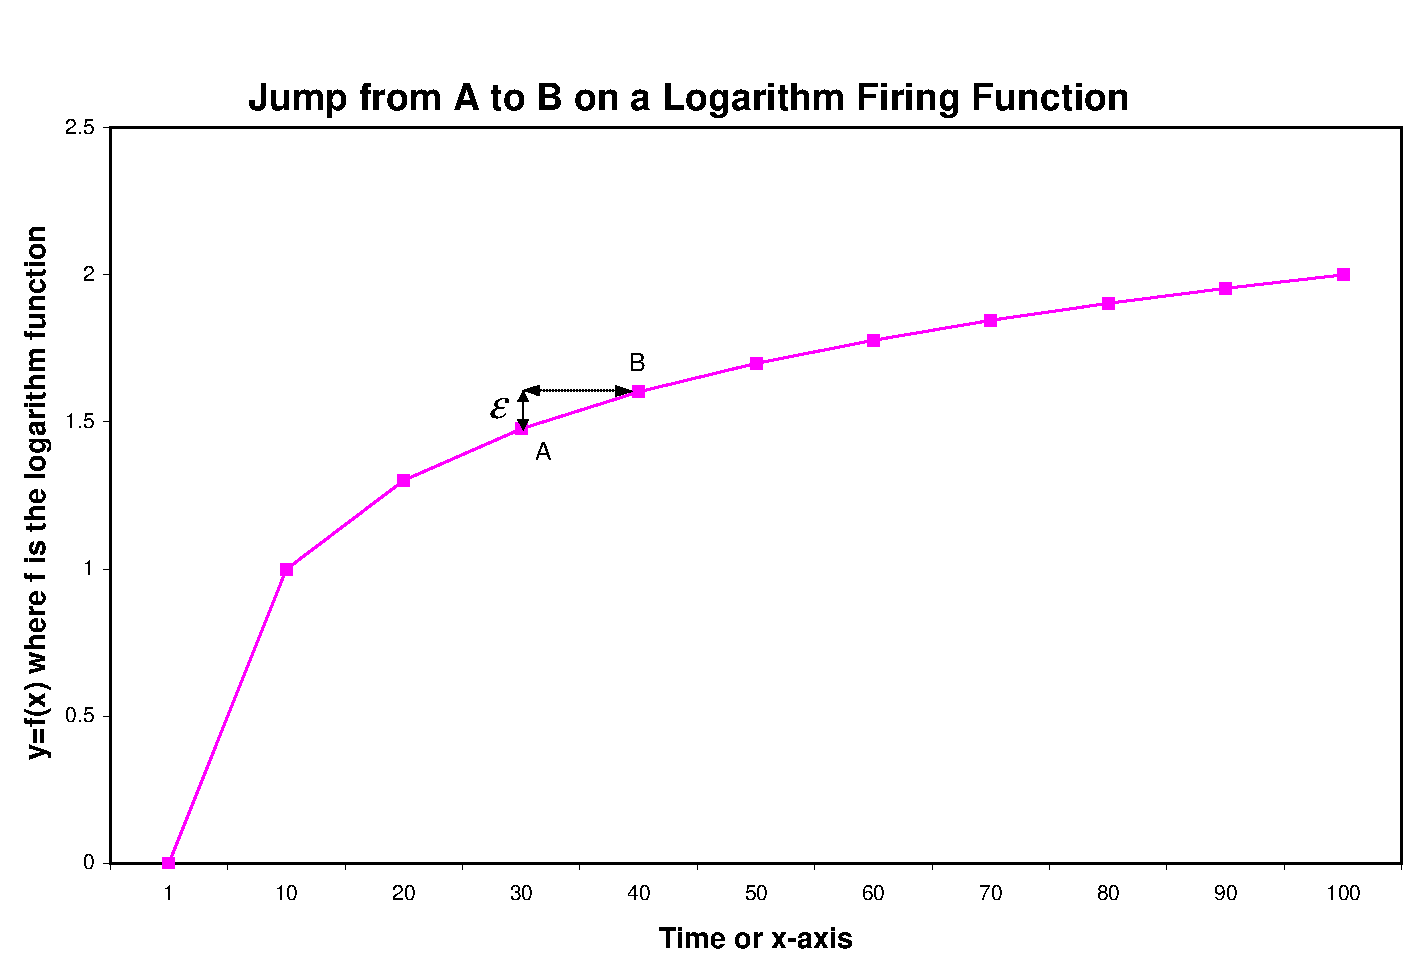
\includegraphics[width=0.9\hsize]{./figures/excelFiringFunc.pdf}
\end{center}
\caption{{\small {\bf A logarithm firing function that displays
a jump from $A$ to $B$ on the curve.}}} 
\label{fig:firingFunc}
\end{figure}

\subsection{The Firefly Synchronization Model}
\label{sec:fireflyModel}

Mirollo and Strogatz extend Peskin's original model for the synchronous
firing of biological oscillators.  Each node in the network is an oscillator
that periodically emits a pulse.  The internal dynamics of the oscillator at
each node, say node $i$, can be generated as a function of a state variable
$x_i(t)$ which takes values within $[0,x_{th}]$, where $x_{th}=1$, is the
threshold value. $x_i(t)$ is a monotonically increasing function that
achieves the threshold value at some time $\tau_i$. Once the threshold is
achieved, the node immediately emits a pulse, $p(t)$ and resets the state
variable to 0, i.e. $x_i(\tau_i^+)=0$.  Mirollo and Strogatz specify that
$x_i$ evolves according to $x_i=f(\phi_i)$, where $f:[0,1]->[0,1]$, is
the \emph{firing function} and it is smooth, monotonic increasing, 
and concave down, i.e., $f'>0$ and $f''<0$.
Here $\phi_i \in [0,1]$ is a phase variable such that, $d\phi / dt = 1/T$,
where T is the cycle period. Furthermore, $\phi_i=0$ when the oscillator is
at its lowest state $x_i=0$, and $\phi_i=1$ at the end of the cycle when
$x_i=1$. Therefore, $f$ satisfies $f(0)=0$, $f(1)=1$.
Fig.~\ref{fig:firingFunc} shows a typical $f$.  The pulses received at each
node will cause an increase to the state variable, thus creating an offset in
the phase of each receiving node.  This effect on the state variable is
called the \emph{coupling} between the transmit and receiver nodes.

Mirollo and Strogatz assume in their model that the oscillators have
identical dynamics, and each is coupled to all the others, and thus has
\emph{all-to-all} communication.  Recent work by Lucarelli and
Wang~\cite{lw04} builds upon this model of pulse coupled oscillators, and
shows that synchronization can be achieved purely on the basis of local
communication, thus discarding the necessity of the all-to-all communication
assumption.


\subsection{The Firing Function}
\label{sec:firingFunc}

The firing function should be monotonically increasing and concave down
according to Mirollo and Strogatz's model.  
Lucarelli and Wang suggest a variety of functions, such as linear, sine, and hyperbolic sine,  
that satisfy this constraint and guarantee synchronization.
Due to the aforementioned resource constraints on the motes, either a very simple linear firing function 
can be selected that does not require floating point arithmetic, or a strategy
is needed to linearize the computation of a non-linear firing function.

The firing function is used to compute the next position, $p_i$ on the 
firing function curve when a pulse or fire is detected. 
Let $(x,y)$\footnote[1]{
We implore the reader to resist the temptation of confusing the $x$ used 
to denote the value on the x-axis in this
context with state variable $x_i$ in section~\ref{sec:fireflyModel}. Although
the notation is confusing, we use $x_i$ to represent the state variable
in order to remain consistent with previous literature that documents Mirollo and Strogatz's model.
}
represent the position of $p_i$ before the fire is detected, 
and let $(x',y')$ represent the new position given that the pulse is detected.
It should be noted that $y$ is not stored explicitly since it can be 
computed using the firing function, $y=f(x)$.
According to Mirollo and Strogatz's model, $y'$ is $y+\epsilon$,
and $x'$ is $f'(y')$ where $\epsilon < 1$ and represents a constant increment in the y axis 
(see Fig.~\ref{fig:firingFunc}), and $f'$ is the inverse of the firing function.
Therefore, in order to implement the model, the inverse of the firing 
function also needs to be computed efficiently.  
We refer to $\frac{1}{\epsilon}$ as the \emph{firing function constant} through
the remaining course of this paper. 

We choose a logarithm function as the firing function.  This is because
apriori it seems that a linear function will be too simple and will not provide
accurate synchronization, and secondly because we can outline a simple
way to linearize the function and compute it efficiently given integer-only
arithmetic that available on the MicaZ sensors. The derivative of $log(x)$ provides a convenient way to linearize
the function in the following way:

\begin{equation}
{dy \over dx}log(x) = {dy \over dx} = {1 \over x}
\end{equation}

\begin{equation}
dy = {dx \over x}
\end{equation}

\begin{equation}
dx = x dy
\end{equation}

The derivative allows us to implement the model in one dimension rather 
than two and does not require computing the inverse of the firing function. 
When a fire is detected, the position of the state variable on the
firing function can be computed by simply multiplying the current $x$ value 
by $dy$, where $dy$ represents $\epsilon$, the firing function constant.
Thus $x' = dx + x$ and $y' = dy + y$.
Evidently, the accuracy of this computation is influenced by the magnitude
of the $dy$ jumps.  In particular, the smaller the $dy$ values, the more accurate will
be the $dx$ value computed. Since the original model defines $\epsilon$ to be
small, specifically $\epsilon < 1$, inaccuracies introduced by using large values
of $dy$ are not a concern in this scheme.


\begin{figure*}[t]
\begin{center}
\begin{tabular}{|p{5cm}|p{3cm}|p{3cm}|p{3cm}|} 
\hline
& {\bf Mirollo and Strogatz} & {\bf Lucarelli and Wang} & {\bf FICA} 
\\ \hline
  {\em \begin{center} Communication Assumptions \end{center}} & 
  {Perfect links and all-to-all communication} & 
  {Perfect links but with only local communication required} &
  {Imperfect, lossy links and only local communication feasible}
\\ \hline
  {\em \begin{center} Event Processing Time \end{center}} &
  {None} &
  {None} &
  {Non-zero, and must be kept to minimum to reduce power and interference
  with other application components}
\\ \hline
  {\em \begin{center} Numeric Precision \end{center}} &
  {Infinite} &
  {Infinite} &
  {Limited by processing exigencies and lack of a floating point unit on the
  ATmega128}
\\ \hline
  {\em \begin{center} Oscillator Dynamics \end{center}} &
  {Perfectly stable oscillators} &
  {Perfectly stable oscillators} &
  {Different crystals on different nodes cause skew, and even on a single
  node environmental factors cause changes over time}
\\ \hline
  {\em \begin{center} Communication Delay \end{center}} &
  {None} &
  {None} &
  {Significant.  Scales with network neighborhood size}
\\ \hline
\end{tabular}
\end{center}
\caption{\small {Differing assumptions used in the different Firefly models.
The breakdown of these assumptions on real hardware nodes required changes to
Strogatz's original model.}}
\label{fig-challenges}
\end{figure*}

\subsection{Implications of Implementing in a Wireless Sensor Network}

Our goal was to implement the Strogatz's Firefly Synchronization model on
networks of MicaZ ''motes''.  The MicaZ is a recent addition to the Mica
family of wireless sensor network devices.  It consists of a 7.3~Mhz
ATmega128L processor, 4KB of SRAM, 128KB of Flash memory for code and data,
and a Chipcon 2420 802.15.4/Zigbee-compliant radio operating at 2.4~Ghz.  The
MicaZ also provides a 51~pin expansion connector allowing integration with
external sensors. The MicaZ runs a small, component-based interface called
TinyOS.  

Table~\ref{fig-challenges} summarizes the main assumptions made in 
the firefly based synchronicity models, and compares this with the conditions
under which we implement FICA.
None of the assumptions made by Mirollo and Strogatz's model can be
upheld in a wireless sensor environment. Noise present in the environment
and packet collisions will introduce error in the routing of simultaneous pulse messages 
between nodes.  Backoff delays introduced by the Medium Access Control (MAC) layer, 
and other radio anomalies extend communication delay and introduce a 
large measure of non-determinism in the time of arrival of pulse messages. 
Furthermore, the all-to-all communication assumption is not feasible 
in multihop networks. Therefore, the demonstration by Wang and Lucarelli~\cite{lw04}
that pulse coupled oscillator based synchronicity can still be achieved 
despite relaxing this assumption forebodes well for the goals of this paper.

Sensor mote hardware also plays a role in violating the assumptions of Mirollo and Strogatz's model. 
Crystal oscillators, are influences by factors such as temperature and humidity, 
and are seldom manufactured identically. Therefore, clock skew is unavoidable in 
the sensor motes since they all tick at different rates. 
This will cause synchronization to degrade as clocks drift apart, and the oscillators
no longer have identical dynamics. Precision will therefore decay as more time elapses between 
synchronization pulses. According to a recent study, typical crystal oscillators
are accurate on the order of one part in $10^4-10^6$~\cite{vig92}, that is two nodes' clocks
will drift apart at $1-100\mu$sec per second.

One of the main changes to Mirollo and Strogatz's model that is introduced
in our implementation is communication delay. In order to address this, we introduce
a delay in processing firing events that are detected by one cycle. This allows
us to efficiently process events in batch mode. Further details of this change
and how we implement it are provided in section~\ref{sec:fitsImplementation}.

Limited computational, energy and memory resources on the motes also constrain
the level of complexity and accuracy of computations that can be performed.
In particular, the absence of floating point arithmetic limits the choice
of a firing function.


\subsection{Implementation Strategy}
\label{sec:fitsImplementation}

\begin{figure}[t]
\begin{center}
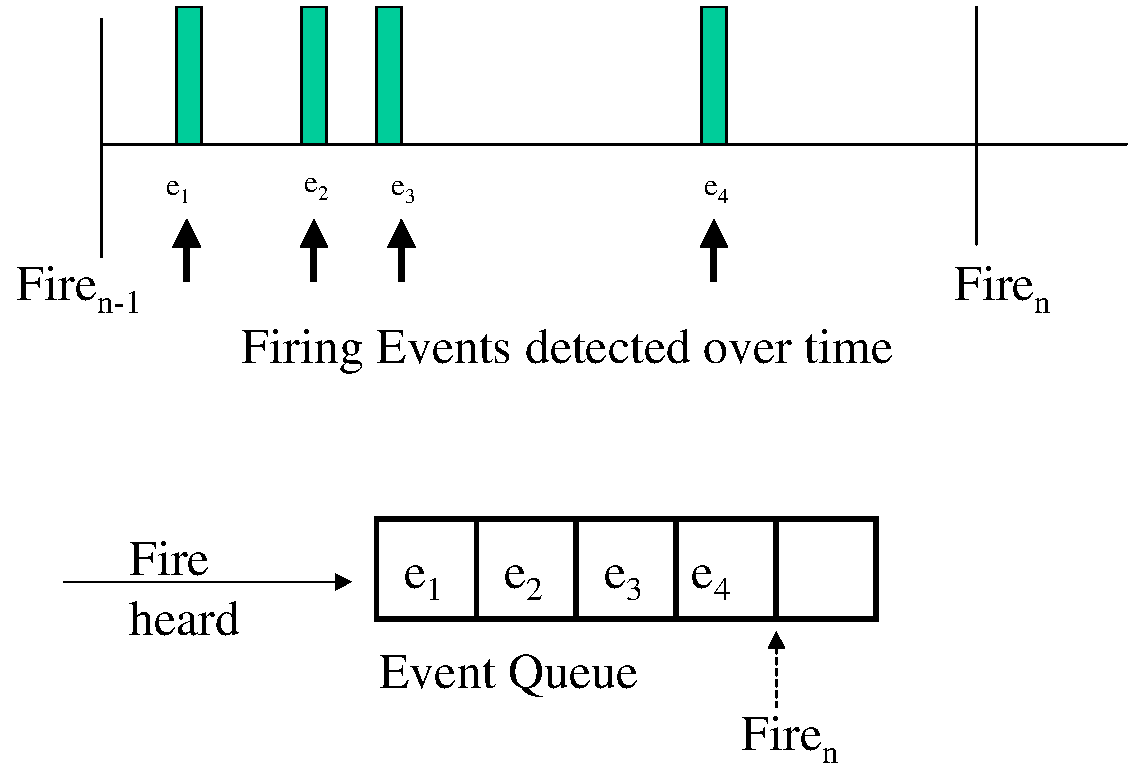
\includegraphics[width=0.9\hsize]{./figures/sortedQueue.pdf}
\end{center}
\caption{{\small {\bf Event Processing: Detected events are stored in a queue sorted by their arrival times and processed at a given time.}}} 
\label{fig:sortedQueue}
\end{figure}

\noindent
In order to address the aforementioned delays introduced by the wireless
sensor network environment, we design an implementation strategy to virtualize time. \\

\noindent
{\bf Processing Events}  \\
In our system each firing event is characterized by 
two messages, the firing message itself and a delay message. 
A firing message contains the sender's local time at
the time it queued the firing message to be sent. A delay message
contains a second timestamp, again using the sender's local
time. The difference between these times represents how long ago the
firing was meant to have occurred. A receiver can then record a firing
event in its own local time by simply subtracting the delay from the
reception time. Each node is assigned a sorted queue to store
detected firing events. The resulting firing event, stored in local time,
is added to the node's sorted queue to be processed later.
All firing events received in one cycle, i.e. received upto a certain amount of 
\emph{idle} time are stored in this queue.  Thus each node remains idle
for a certain period of $\delta(t)$ time, during which it receives and records
firing events. When this idle period is over, the node begins to process the queued events.
Fig.~\ref{fig:sortedQueue} illustrates the queue-based approach of storing
and processing firing events.

Each time a node fires, the next time it will fire can be computed
based on the firing events it detected thus far that are 
stored in the sorted queue.

The tradeoff of the virtualized time strategy is that the response to firing events
is no longer in real time. Firing events detected impact the next firing cycle rather than
the current one. For instance in the first cycle, there are no events in the queue.
Thus, we program the nodes to remain idle by simply storing and processing the events
they detect during this first cycle.

We take a moment to digress to detail a caveat introduced by our hardware
platform. The radio stack on the MicaZ sensor motes, CC2420, does not
permit including the delay message in the same packet as the firing message.
Therefore, two messages are necessary.\\

\noindent
{\bf Computing Next Firing Time}  \\
A node moves closer to firing based on two factors: detecting a firing
and the passing of time. When a firing event is dequeued, the amount of 
elapsed time since the last event recorded is noted.
The represents the time spent waiting without detecting any event. 
This interval is added to the current time, and the magnitude of the jump
on the firing function is computed. This jump is added to the node's 
current time.

In order to implement this, two notions of time need to be tracked:
wall clock time,  which represents the time elapsed between processing
events, as well as the value on the x-axis of the node's current
position on the firing function. \\

\noindent
{\bf 'Ignore-period' For Addressing Pulse Additivity Issues}  \\
Initial experiments showed that on a 15 nodes fully connected graph,
the nodes split into two groups where each individual group achieves synchronicity
amongst its members, but does not achieve synchronicity with the other group.
We believe one reason could be that the additive effect of multiple firings
from the neighboring group is preventing the group from synchronizing with
that group. In order to correct for this \emph{additivity} issue, we 
introduce an \emph{ignore-period} which characterizes the amount of time
during which a node just drops detected events rather than processing
them or storing them in a queue.  Since the ignore-period period may
not be the best solution for the additivity issue, we have implemented
it in a select number of experiments, to determine its effectiveness
in addressing the pulse additivity issues.





 
%\input{design.tex} 
%\input{implementation.tex}
\section{Evaluation}
\label{sec:evaluation}

We have performed experiments both on MicaZ sensors that are part of Motelab, a 38 node
cluster of MicaZ sensors deployed in the Harvard Computer Science building,
as well as performed a variety of simulations on TOSSIM, a TinyOS mote simulator~\cite{hill00}.

\subsection{TOSSIM}
There are several aspects of TOSSIM that make it an unrealistic testbed for
our algorithm which we want the reader to be aware of.
TOSSIM's bit-level radio stack is based on the RFM1000 chip 
which is completely different from the CC2420 in the MicaZ sensors on motelab. 
Thus TOSSIM's radio model is unrealistic for our purposes, 
and furthermore does not currently capture clock skew.  
Additionally, TOSSIM does not model processor time well: 
computation always takes zero time, regardless of the number of instructions, 
and interrupts are instantaneous.
On the the other hand, TOSSIM allows convenient,
direct experimentatation by allowing the user to specify arbitrary topologies, 
and scales to thousands of nodes. Additionally TOSSIM allows addition of user
defined \emph{printfs} to the code which makes debugging a lot simpler
than it is on Motelab.  

In spite of TOSSIM's limitation as a realistic testbed, we choose to 
devote a large part of our evaluation to TOSSIM experiments because it
allows convenient exploration of the parameter space of FICA, our
firefly-based synchronicity scheme. One of our underlying goals is to
throughly explore our synchronicity scheme's parameter space and 
ensure that it is accurate in an ideal testing environment such as TOSSIM.
This will portend well for the effectiveness of our scheme on Motelab, where
testing and debugging is laborious.  It should be noted that attempts to
build clock skew into TOSSIM are currently underway. \\

\subsection{Evaluation Criteria}
\noindent
We focus on two main criteria for evaluating the level of synchronicity achieved:
\begin{enumerate}\addtolength{\itemsep}{-0.5\baselineskip}
\item What is the time taken to achieve synchronicity amongst a group of nodes?
\item How stable is the level of synchronicity achieved?
\end{enumerate}

We define a \emph{period} as the time between firings of two nodes.
For a group of nodes, a period is defined as the time between firings of the
members of that group, where the firings are computed as the
average of the individual mote firings of the group members.
We classify \emph{stability} in terms of consistency of membership 
in a group of sychronized nodes, as well as the consistency of 
the period of the nodes in that group. 
A single group of nodes with a constant number of members, and with a 
regular period, characterizes effective synchronicity. \\

\noindent
{\bf Detecting Groups of Synchronized Nodes} \\
Initial experiments on TOSSIM indicate the possibility
of nodes splitting into separate groups of synchronized entities.
Therefore we have designed our metrics to process data for 
more than one group of synchronized nodes.

In order to detect groups, we have adopted a moving window approach.
In this approach nodes that consistently remain coupled within a certain time period
are grouped together. Given a fixed user-defined window size, the algorithm
finds the best set of motes that fire within that window and 
identifies them as one group. 
This window \emph{moves} over time, and as more firing events are detected, 
group membership is updated.
This is a fairly complex algorithm, and difficult to implement correctly.
Due to space constraints, we do not provide any further details,
and encourage the reader to look at our code repository for a detailed
description of the algorithm.

\subsection{Evaluation Metrics}
We defined the following metrics to evaluate synchronicity in our experiments:

\begin{enumerate}

\item {\bf Group Period}: This measures the length of the period between
which nodes in a group fire.  It is particularly useful to see how the
group period varies with time. Significant variation in a synchronized 
group's period over time will prevent time from advancing uniformly, and
hinders the use of synchronicity for serving as a time synchronization
scheme.

\item {\bf Group Spread}: This measures the extent of variation of 
firing of individual nodes in a group.  This metric captures the precision
of the synchronicity achieved by the nodes.
The standard deviation of the various firing times of the members of group
provides an estimate of how far apart their firing times are.

\item {\bf Time to Achieve Synchronicity}: This measures the 
amount of time it takes for all the nodes in a group to fire 
simultaneously. This metric captures the speed at which synchronicity
is achieved and thus reflects to some extent on the efficiciency of 
our scheme.  Achieving fast synchronicity is crucial for the aforementioned
applicatons in sensor nodes such as power scheduling and coordinated 
data collection.  Whether synchronicity is achieved at all is implicit
in this measure.
This metric is computed by measuring the amount of time taken by 
a certain percentage of motes to form a group and remain in that group
for a certain number of periods.

\item {\bf Group Membership: Nodes entering and exiting}: 
For debugging purposes, it is important to be able to examine 
the membership of individual nodes in a group, and be able to detect whether
group members are being lost, or whether random group members are being
deleted or whether duplicate group members exist.
We use this metric as a means of debugging our 
synchronicity implementation. For a given experiment, this metric
provides a reliable means of determining and verifying 
the quality of group membership.  
\end{enumerate}

\begin{table}
\centering
\caption{Time taken to synchronize (in seconds) for 16 nodes in TOSSIM with different grid topologies, and different values of firing function constants (FFC). The - indicates cases in which synchronization is not achieved.} 
\label{tab:topologyFFC}
%%\subfigure[Table 1: Number of element]
\vspace{2pt}
\begin{tabular}{|r|r|r|r|r|} \hline
Topology                & {\bf FFC=10}  & {\bf FFC=50} & {\bf FFC=100} &   {\bf FFC=200}  \\ \hline
{\bf Grid}              &   90.70    &   73.55     &   84.24        &   266.89      \\ 
{\bf Ring}              &   -        &  123.55     &   77.87        &   194.83      \\ 
{\bf All-To-All}        &   98.43    &   23.44     &   59.35        &   227.05      \\ 
{\bf Line}              &   83.97    &   183.94    &   219.42       &   456.62      \\ \hline
\end{tabular}
\end{table}
\begin{table}
\centering
\caption{Average and Standard Deviation Statistics Per Topology for Table~\ref{tab:topologyFFC}.}
\label{tab:topologyStat}
%%\subfigure[Table 1: Number of element]
\vspace{2pt}
\begin{tabular}{|r|r|r|r|r|} \hline
Topology                & Average    & Standard Deviation \\ \hline
{\bf Grid}              & 128.85     & 92.30 \\ \hline  
{\bf Ring}              & 135.42     & 58.50  \\ \hline  
{\bf All-To-All}        & 102.07     & 88.77  \\ \hline  
{\bf Line}              & 235.99     & 157.87 \\ \hline  
\end{tabular}
\end{table}

\begin{figure}
\begin{center}
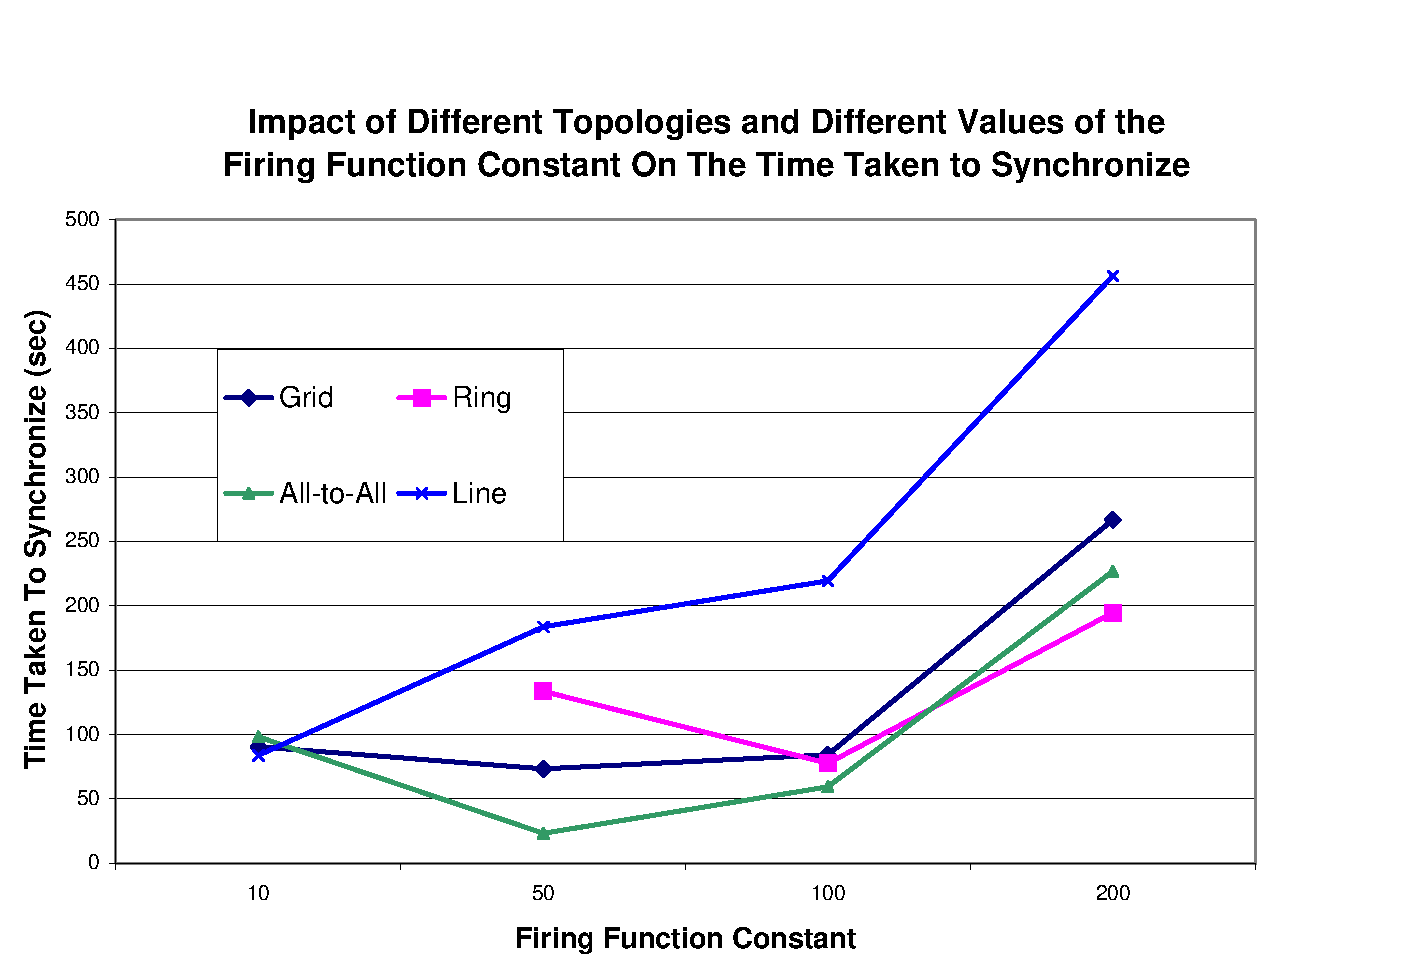
\includegraphics[width=1.1\hsize]{./figures/topFFC.pdf}
\end{center}
\caption{{\small {\bf The impact of topology and the magnitude of the firing function constant on the time to synchronize.
The exact values of the time taken to synchronize are listed in~\ref{tab:topologyFFC}.}}} 
\label{fig:topFFC}
\end{figure}

\begin{figure}[t]
\begin{center}
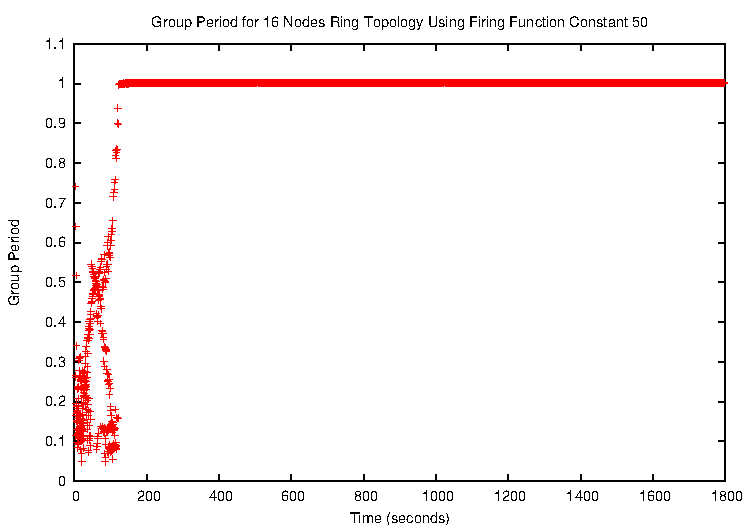
\includegraphics[width=1.0\hsize]{./figures/5-Jan-2005-1-RING-NODES-16-50CONSTANT-GROUP-PERIOD.pdf}
\end{center}
\caption{{\small {\bf Group period for 16 node ring topology with firing function constant 50.}}} 
%{\em This figure shows...}}}
\label{fig:rgp}
\end{figure}

\begin{figure}[t]
\begin{center}
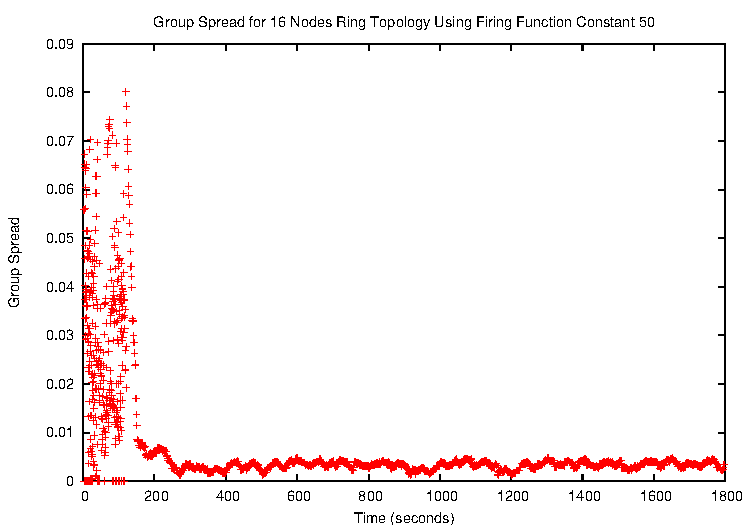
\includegraphics[width=1.0\hsize]{./figures/5-Jan-2005-1-RING-NODES-16-50CONSTANT-GROUP-SPREAD.pdf}
\end{center}
\caption{{\small {\bf Group spread for 16 node ring topology with firing function constant 50.}}}
%{\em This figure shows...}}}
\label{fig:rgs}
\end{figure}

\begin{figure}[t]
\begin{center}
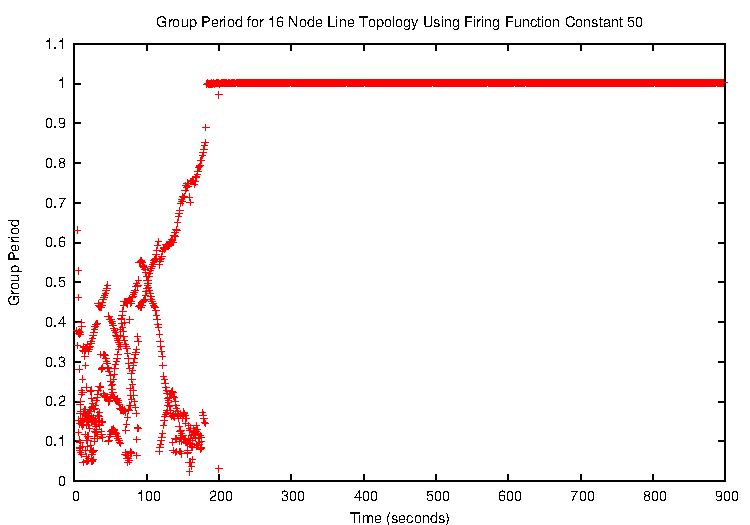
\includegraphics[width=1.0\hsize]{./figures/5-Jan-2005-1-LINE-NODES-16-50CONSTANT-GROUP-PERIOD.pdf}
\end{center}
\caption{{\small {\bf Group period for 16 node line topology with firing function constant 50.} }}
%{\em This figure shows...}}}
\label{fig:lgp}
\end{figure}

\begin{figure}[t]
\begin{center}
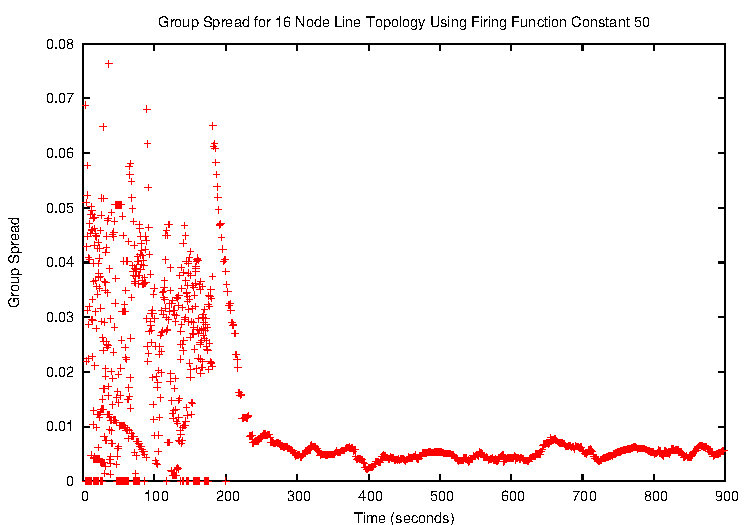
\includegraphics[width=1.0\hsize]{./figures/5-Jan-2005-1-LINE-NODES-16-50CONSTANT-GROUP-SPREAD.pdf}
\end{center}
\caption{{\small {\bf Group spread for 16 node line topology with firing function constant 50.} }}
%{\em This figure shows...}}}
\label{fig:lgs}
\end{figure}

\begin{figure}[t]
\begin{center}
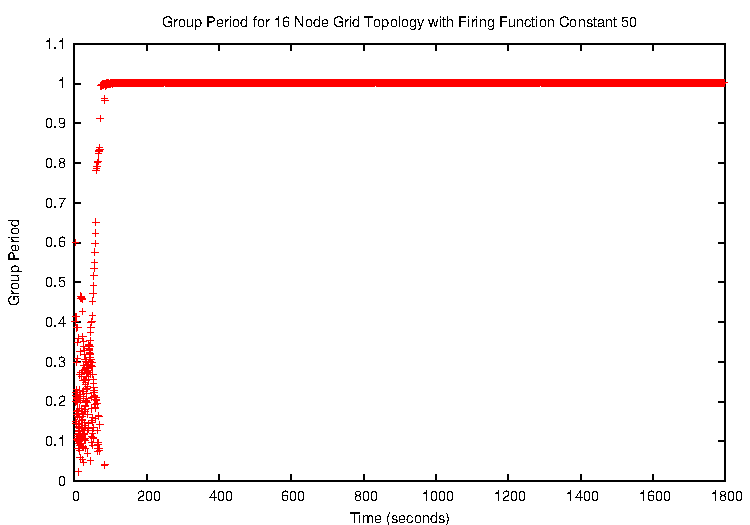
\includegraphics[width=1.0\hsize]{./figures/5-Jan-2005-1-GRID-NODES-16-50CONSTANT-GROUP-PERIOD.pdf}
\end{center}
\caption{{\small {\bf Group period for 16 node 4by4 regular grid topology with firing function constant 50.} }}
%{\em This figure shows...}}}
\label{fig:ggp}
\end{figure}


\begin{figure}[t]
\begin{center}
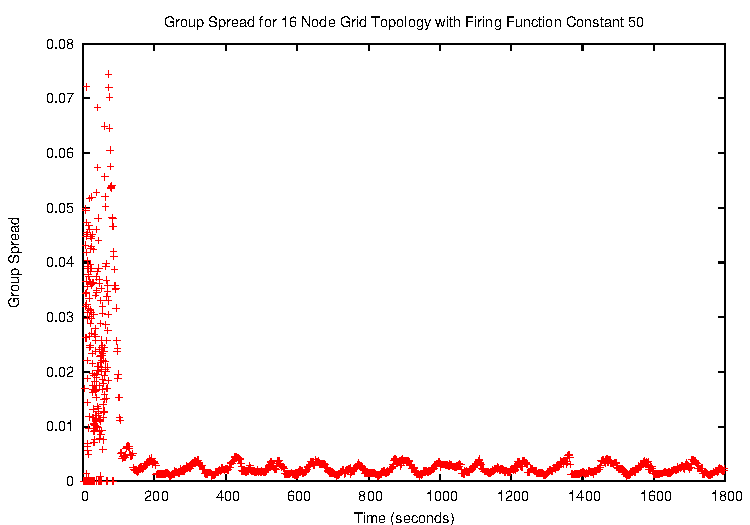
\includegraphics[width=1.0\hsize]{./figures/5-Jan-2005-1-GRID-NODES-16-50CONSTANT-GROUP-SPREAD.pdf}
\end{center}
\caption{{\small {\bf Group spread for 16 node 4by4 regular grid topology with firing function constant 50.} }}
%{\em This figure shows...}}}
\label{fig:ggs}
\end{figure}


\begin{figure}[t]
\begin{center}
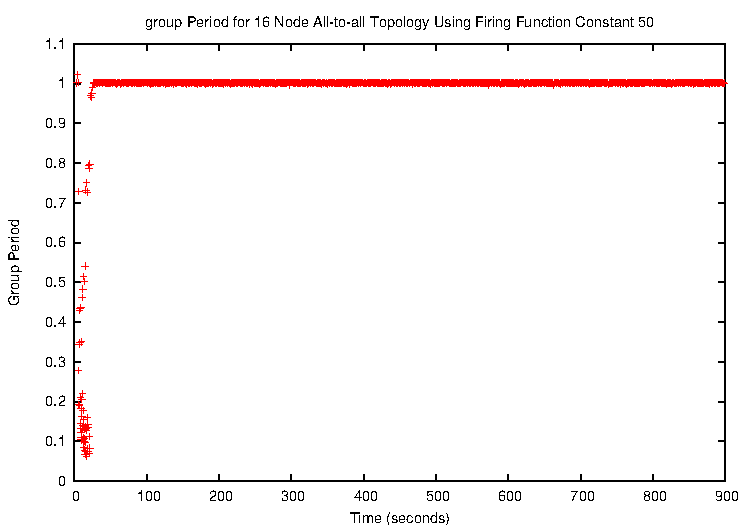
\includegraphics[width=1.0\hsize]{./figures/5-Jan-2005-1-ALL-NODES-16-50CONSTANT-GROUP-PERIOD.pdf}
\end{center}
\caption{{\small {\bf Group period for 16 node all-to-all topology with firing function constant 50.} }}
%{\em This figure shows...}}}
\label{fig:agp}
\end{figure}

\begin{figure}[t]
\begin{center}
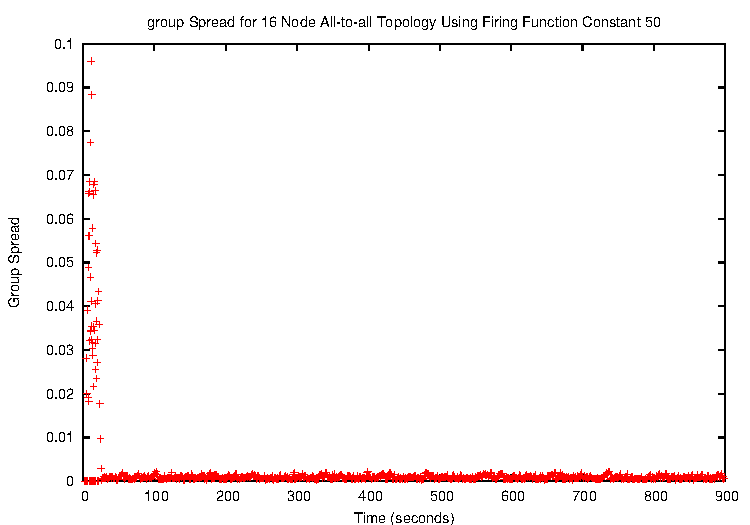
\includegraphics[width=1.0\hsize]{./figures/5-Jan-2005-1-ALL-NODES-16-50CONSTANT-GROUP-SPREAD.pdf}
\end{center}
\caption{{\small {\bf Group spread for 16 node all-to-all topology with firing function constant 50.} }}
%{\em This figure shows...}}}
\label{fig:ags}
\end{figure}




\subsection{TOSSIM Experiments}
A number of simulation experiments have been performed on TOSSIM to evaluate
the impact of different parameters of the model on the accuracy and
quality of synchronicity achieved amongst the nodes.  We explore the impact
of parameters such as the firing function constant (a constant value that
is equal to $\frac{1}{\epsilon}$, where $\epsilon$ is the firing function
related quantity discussed in sections~\ref{sec:fireflyModel} and ~\ref{sec:firingFunc}), 
and the number of nodes on the quality of synchronicity achieved as 
measured by group spread, group period and time taken to synchronize.

Fig.~\ref{fig:topFFC} shows the values of time to synchronize for 16 nodes with different
topologies and firing function constants.  It is obvious that a higher firing function
constant does not imply consistently lower time to synchronization.  Overall nodes in the
line topology takes the longest time to synchronize except when the firing function constant
is 10. 
Nodes in the all-to-all topology generally take less time to synchronize than the other
topologies. This is not surprising since all-to-all is the best conceivable topology.
Tables~\ref{tab:topologyFFC}-~\ref{tab:topologyStat} show numerical values of the
time taken to synchronize (in seconds) for different topologies and firing function
constant values. The standard deviations give an idea of the large extent to
which the firing function constant can influence the time taken to achieve synchronicity.
In Table~\ref{tab:topologyStat} the line topology has the highest standard deviation,
and indicates that this topology is particularly vulnerable to changes in the firing function
constant.

Fig.~\ref{fig:rgp}-~\ref{fig:ags} show the group period and group spread of 16 nodes
with four different topologies: line, 4by4 regular grid, ring and all-to-all.
It is reassuring to see that for all node topologies, the group period stabalizes
at 1 after a given time period.  The group period of the line topology takes the
longest time to stabalize (190 seconds), while the group period of the all-to-all topology 
takes the shortest amount of time to stabalize (less than 30 seconds). Similarly
the group spread of the all-to-all topology has the least amount of variation,
and the group spread of the line topology has the most amount of variation.
The reason for this is quite intuitive. In the line topology, nodes towards the ends
of the lines have difficulty detecting all the fires. On the other hand, nodes in the
all-to-all connected topology are well connected to all their neighbors and
can efficiently respond to detected fires.


%% Geoff's graphs here

\begin{figure}[t]
\begin{center}
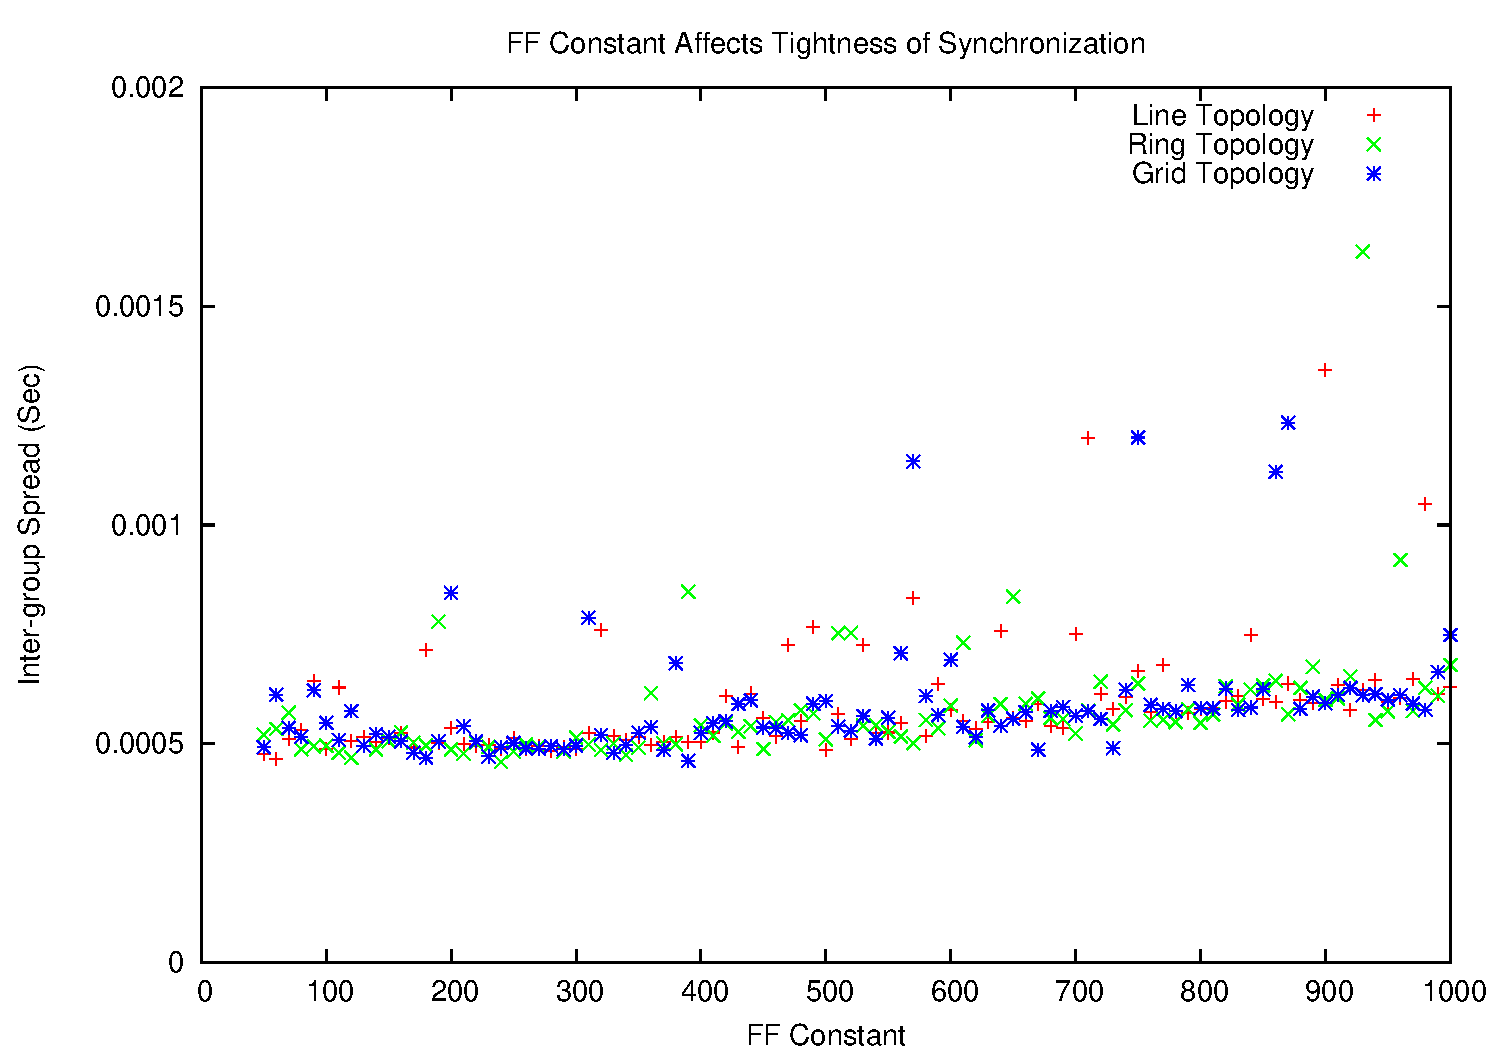
\includegraphics[width=1.0\hsize]{./figures/16-NOADD-LINERINGGRIDALLALL-SPREAD.pdf}
\end{center}
\caption{{\small {\bf The impact of the firing function constant on the group spread for three different node topologies}}}
\label{fig:lgp}
\end{figure}

\begin{figure}[t]
\begin{center}
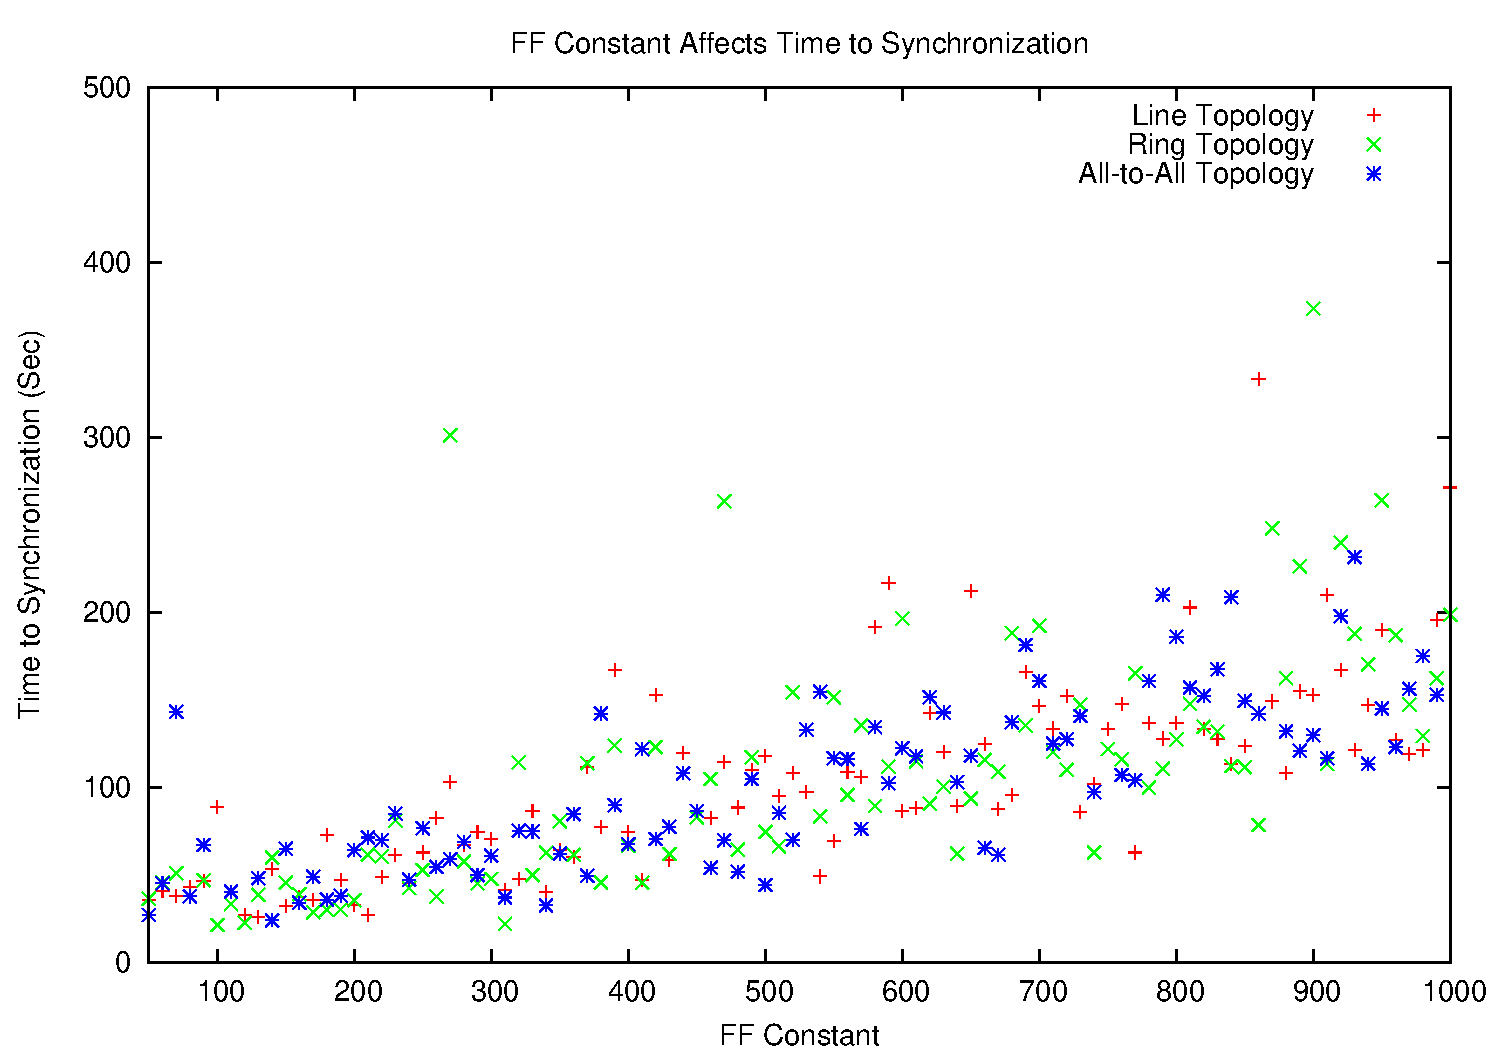
\includegraphics[width=1.0\hsize]{./figures/16-NOADD-LINERINGALLTOALL.pdf}
\end{center}
\caption{{\small {\bf The impact of the firing function constant on the time taken to synchronize for three different node topologies.}}}
\label{fig:lgp}
\end{figure}

\begin{figure}[t]
\begin{center}
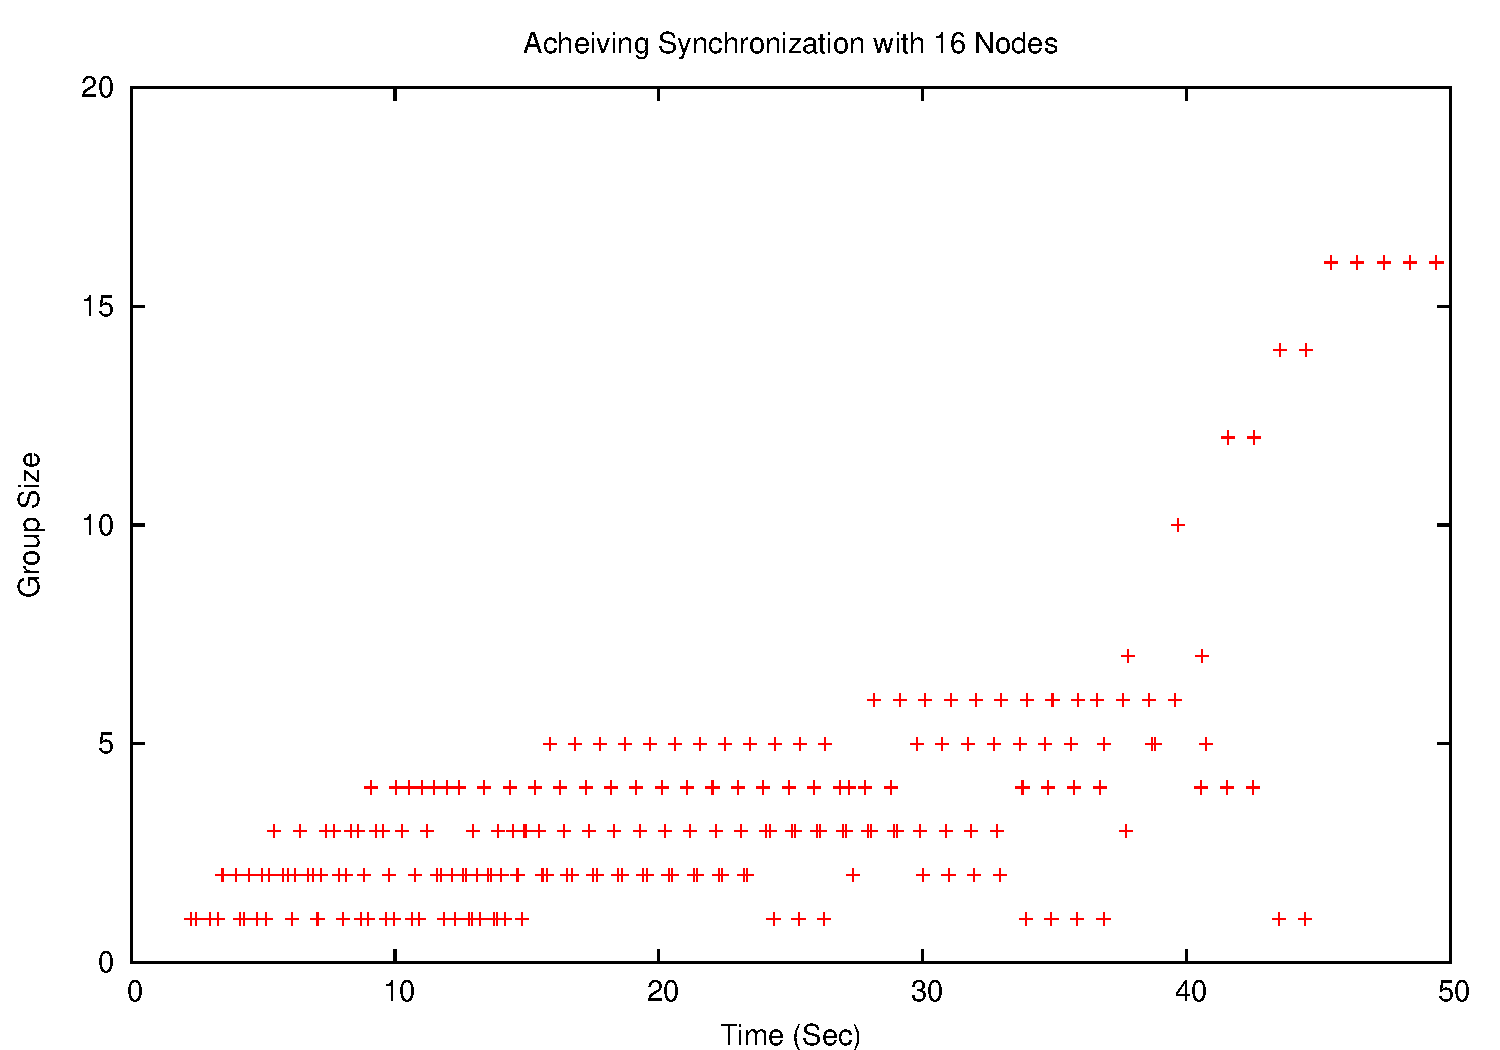
\includegraphics[width=1.0\hsize]{./figures/11-Jan-2005-1-16MOTES-150CONSTANT-RING-EVENT-ALL-GROUPS.pdf}
\end{center}
\caption{{\small {\bf The size of a group over time.}}}
\label{fig:lgp}
\end{figure}



\section{Discussion}
\label{sec:discussion}

In the course of developing FICA we have encountered a number of difficulties
inherent in moving distributed algorithms from mathematical simulation on to
realistic platforms.  Additionally, we have had time to track the
always-interesting dynamics of FICA over a large parameter space.  This
section collects a set of disparate remarks and observations we made during
the course of development and analysis.

\subsection{Sensor Node Hardware Limitations and Changes}

Any algorithm aiming for microsecond-level accuracy in wireless sensor
networks has aligned its fate with the capabilities of the underlying
harwarde platform.  Low-level hardware changes can cause large problems.
Two examples from FICA illustrate this, and elucidate the consequences of
subtle differences between the Mica2, MicaZ, and Telos ''motes''.

First, as discussed earlier, when operating on MicaZ's or Telos FICA is
forced to send two radio messages corresponding to each fire.  The receival
of the first message marks the fire time in the receiver's context, but it is
the second message that contains the sender's delay that allows the receiver
to extrapolate backwards in it's own time frame.  If deployed on Mica2's,
however, FICA could send only one message, since the older Chipcon CC1000
radio stack maintained the contents of the packet in memory which allowed
rewriting up to the moment of, and even during, message transfer.  The newer,
in most ways better CC2420 radios operate at a packet level.  Since message
contents are copied into the radio buffer at send time they cannot modified
during flight, an interesting consequence of moving the software/hardware
boundary.

Second, FICA requires accurate event timestamping.  On the MicaZ and Mica2,
which share the ATMega128 processor, counters can be run up to the clock
speed of ~8MHz allowing fine-grained precision.  Unfortunately the HP chips
used in the Telos ''motes'' do not appear to have cycle counters that can run
at this speed, an omission surely to be noticed by those developing time
synchronization algorithms.

\subsection{Effects of Additivity}

As discussed earier, in response to the 2-group convergences seen in early
simulations we modified our implementation to elimininate additivity.  By
this we refer to treating a group of firing events clustered close-enough
together in time as a single fire.  At the time we thought that this was a
reasonable solution and a workaround to the discretized time present on our
hardware platform that differs from the continuous time presented in the
Lucarelli and Strogatz models.

Later, after running a large number of simulations with this no-addivity
codebase and seeing many cases of non-convergence, we began to suspect that
the earlier 2-group solutions that we had seen were the result of either an
inappropriate choice of our firing function constant (which is directly tied
to the delta of the Strogatz model, required to be small compared with the
firing interval) or a change to the dynamics of the model introduced by not
processing events continuously.  After reintroducing the additive effects we
were able to run a small set of simulations with large numbers of nodes and
more reasonable firing function constants which produced the very encouraging
results found graphed in this paper.

\subsection{Challenges Evaluating on MoteLab}

While we had original planned to deploy and evaluate FICA on MoteLab we found
the second half of that exceedingly difficult to do.  Although MoteLab is a
powerful tool for doing many types of sensor network experimentation it was
difficult to design a simple experiment that would allow us to verify the
correct functioning of the FICA system.

Early investigations conducted on MicaZ's were done with the nodes in visual
range, allowing inspection of the leds blinked on firing events to suffice as
evidence of synchronicity.  With 30 nodes sprinkled throughout offices and
labs, MoteLab obviously does not lend itself to such an approach.  Having
each node log its firing times is also untenable as the clock skew across
nodes would make it impossible to ascertain synchronicity after a brief
period of time.

Our initial approach was to remove a certain set of nodes from the experiment
to serve as passive listeners.  These nodes ran a modified version of the
{\tt TOSBase} code in the TinyOS tree.  When a passive listener
receives a message it timestamps it low in the radio stack.  These times are
logged to the database and should allow the firings of nearby nodes to be
reconstructed viewed through the receiver's time frame.

Though seemingly plausible the approach described above does not work well,
for a variety of reasons, mainly due to difficulties introduced
in post-processing by lossy links and multi-path effects.  We will continue
to develop our post-processing tools to try and deal the much messier data
produced by MoteLab, but other solutions may be possible.  One approach may
be to, in a seperate experiment, build up a model of the clock skew of each
node in our testing array.  If the clock frequency is relatively stable on
each node over time, such a model would allow data collected on each node to
be converted into a global time scale and thus compared with other nodes.
Another out-of-band solution would be backchannel boards capable of
timestamping radio events without disturbing node operation.

\subsection{Reducing Resource Usage}

Mindful that any synchonicity system will serve as a tool for other software
components in a sensor network application doing real work, we have begun to
consider ways to reduce the bandwidth and energy consumption of FICA.

Currently FICA sends radio packets and does some processing each second.  In
networks attempting to collect and move data the bandwidth overhead is
especially prohibitive.  One way to reduce the bandwidth consumed by FICA
would be to reduce the firing frequency.  Using the known properties of the
node oscillators and given the synchronicity requirements of a given
application an appropriate minimum firing frequency could be calculated.

Unfortunately reducing the firing frequency has the side effect of increasing
the time to synchronization, which may be unacceptable in systems expected to
deploy and respond to topology changes quickly.  One possible solution is to
have the network itself recognize when it has achieved a given level of
synchronicity and throttle down the firing frequency.  Another, somewhat
orthogonal solution would be to let individual nodes choose to skip firing
events, perhaps again based on a local perception of how in step they were
with their neighbors.

\section{Conclusions and Future Work}
\label{sec:conclusion}

Designing a synchronicity scheme for wireless sensors
is particularly challenging in light of the resource and computation 
constraints on these devices. In this paper we
designed and implemented FICA, a firefly-based synchronicity mechanism 
for a wireless sensor platform.

A firefly based synchronicity scheme has several salient features.  
The underlying algorithm derived from Mirollo and Strogatz's original model 
of pulse-coupled integrate and fire dynamics is simple to implement and 
requires little parameter tweaking.  On the other hand, the evaluations
in this paper expose several weaknesses of this scheme. 
Our experiments indicate the sensitivity of our synchronicity scheme 
to factors such as the firing function constant and number of nodes in the network.
While the impact of node topology on the quality of synchronicity attained
is not surprising, it exposes yet another vulnerability of our scheme.
Furthermore, the scheme requires constant message exchange in the form 
of sending and receiving pulses, and makes strong demands on
bandwidth and energy, resources which are extremely constrained on sensor nodes.
Finally, it is not immediately clear how to make a number of pulse-coupled 
nodes synchronize to an external timescale such as GPS. This functionality,
if possible, could serve many different applications.

There are several avenues of future work that could be pursued. 
Our primary future goal is to resolve the issues we currently face with implementing
FICA on MicaZ nodes in Motelab, and be able to test the quality of our synchronicity
scheme in this real world setting.
It would be useful to perform a detailed study of the power requirements of 
implementing our synchronicity mechanism on wireless sensors and 
to quantitatively evaluate its operational demands.





%%%%%%%%%%%%% BIBLIOGRAPHY %%%%%%%%%
\begin{small}
\bibliographystyle{abbrv} \bibliography{paper}
\end{small}

\end{document}

